\documentclass[12pt]{article}

\usepackage{sbc-template}
\usepackage[utf8]{inputenc}
\usepackage{amsmath}
\usepackage{amssymb}
\usepackage{graphicx}
\usepackage{booktabs}
\usepackage{url}
\usepackage{microtype}
\usepackage{enumitem}

% Compactacao estrita de listas e espacamento para orcamento rigoroso de 7-8 paginas
\setlist{nosep,topsep=1pt,partopsep=0pt,parsep=0pt,leftmargin=1.2em}
\renewcommand{\topfraction}{0.95}
\renewcommand{\bottomfraction}{0.90}
\renewcommand{\textfraction}{0.05}
\renewcommand{\floatpagefraction}{0.85}
\setlength{\floatsep}{3pt plus 1pt minus 1pt}
\setlength{\textfloatsep}{4pt plus 1pt minus 1pt}
\setlength{\intextsep}{3pt plus 1pt minus 1pt}
\setlength{\abovecaptionskip}{2pt}
\setlength{\belowcaptionskip}{2pt}
\setlength{\abovedisplayskip}{2pt plus 1pt minus 1pt}
\setlength{\belowdisplayskip}{2pt plus 1pt minus 1pt}
\setlength{\abovedisplayshortskip}{1pt plus 1pt}
\setlength{\belowdisplayshortskip}{1pt plus 1pt}
\setlength{\parskip}{1.5pt plus 0.4pt minus 0.4pt}

% Otimizacao do ambiente thebibliography para padrao SBC compacto
\let\oldthebibliography\thebibliography
\let\endoldthebibliography\endthebibliography
\renewenvironment{thebibliography}[1]{%
  \begin{oldthebibliography}{#1}%
    \setlength{\itemsep}{0pt plus 0.2pt}%
    \setlength{\parskip}{0pt}%
    \footnotesize
}{%
  \end{oldthebibliography}%
}

\title{Do Simbólico à Incerteza: Pipeline Integrado de Inteligência Artificial para Predição e Mitigação do Atraso Crítico na Notificação Vacinal do PNI}

\author{Autor 1\inst{1}, Autor 2\inst{1}, Autor 3\inst{1}}

\address{Departamento de Ciência da Computação -- Universidade Federal do Amazonas (UFAM)\\
  Manaus -- AM -- Brasil
  \email{\{autor1, autor2, autor3\}@icomp.ufam.edu.br}
}

\begin{document}

\maketitle

\begin{resumo}
A notificação tempestiva no Programa Nacional de Imunizações (PNI/MS) é essencial contra a cegueira epidemiológica. Investigamos 15.403 registros reais do PNI via RNDS/DATASUS, modelando o atraso crítico ($>7$ dias, 51,59\% da base) em seis etapas de IA: indução de árvore ID3, modelos lineares com Ridge e regressão logística, teoria axiomática da probabilidade com diagnóstico bayesiano, Naive Bayes com recuperação de regimes operacionais latentes via Expectation-Maximization (EM), modelagem causal por Redes Bayesianas com colisor e d-separação, e lógica Fuzzy Mamdani acoplada à probabilidade a posteriori para triagem contínua no SUS. A inclusão da variável latente eleva a acurácia de 75,79\% para 93,77\%, e a rede causal reduz em 67,74\% a parametrização conjunta, gerando subsídios operacionais interpretáveis.
\end{resumo}

\begin{abstract}
Timely reporting in Brazil's National Immunization Program (PNI/MS) is vital against epidemiological blindness. We analyze 15,403 sanitized records from RNDS/DATASUS, modeling critical delay ($>7$ days, 51.59\% of data) across a six-stage AI pipeline: ID3 decision tree induction, linear models with Ridge and logistic regression, axiomatic probability theory and Bayesian diagnostics, Naive Bayes with latent regime recovery via Expectation-Maximization (EM), causal Bayesian Networks with collider and d-separation analysis, and Mamdani Fuzzy logic fed by Bayesian posteriors for continuous SUS triage. Introducing latent regimes increases accuracy from 75.79\% to 93.77\%, and causal factorization yields 67.74\% parameter savings, delivering interpretable public health decision support.
\end{abstract}

\section{Introdução e Contexto Epidemiológico}

A vigilância epidemiológica contemporânea depende da integridade e tempestividade dos registros vacinais. No Brasil, o Programa Nacional de Imunizações (PNI), sob gestão do Ministério da Saúde e do DATASUS, consolida imunizações em escala nacional através da Rede Nacional de Dados em Saúde (RNDS) \cite{brasil2023pni}. Entretanto, disparidades regionais de infraestrutura tecnológica entre capitais e postos remotos geram represamentos operacionais severos entre a data de aplicação da vacina e sua inserção efetiva no sistema central.

Esse represamento produz a chamada ``cegueira epidemiológica'', distorcendo estimativas de cobertura vacinal em tempo real e atrasando respostas a surtos infecciosos. A questão investigada neste trabalho é: \textit{Quais determinantes técnicos governam a latência vacinal no SUS, e como sistemas de IA combinando métodos simbólicos, lineares, probabilísticos e fuzzy podem predizer e mitigar o atraso crítico de notificação?}

Utilizou-se uma base de $N = 15.403$ registros higienizados do PNI da plataforma de Dados Abertos do DATASUS. A latência contínua é definida por $\Delta t = \text{dt\_entrada} - \text{dt\_vacina}$, expressa como \texttt{dias\_atraso}. A partir dela, formulou-se a variável-alvo binária primordial:
\begin{equation}
Y = \text{atraso\_critico} = 
\begin{cases}
1, & \text{se } \Delta t > 7,0 \text{ dias} \\
0, & \text{se } 0 \le \Delta t \le 7,0 \text{ dias}
\end{cases}
\end{equation}
Na base analisada, há $7.947$ ocorrências de atraso crítico ($51,59\%$) e $7.456$ oportunas ($48,41\%$), configurando um cenário amostral equilibrado para modelagem preditiva.

\section{Arquitetura Geral do Pipeline Integrado}

Para mitigar a incerteza e a complexidade empírica dos microdados do SUS, estruturou-se um pipeline integrado de seis etapas (Figura~\ref{fig:pipeline}). O encadeamento conecta: (1) indução simbólica ID3 para seleção de atributos relevantes e extração de regras; (2) regressão OLS, multivariada com regularização Ridge e baseline logístico; (3) formalização da probabilidade axiomática de Kolmogorov, tabela conjunta e inversão diagnóstica de Bayes; (4) aprendizado probabilístico com Naive Bayes e descoberta de regimes latentes via algoritmo EM; (5) DAG causal com estrutura de colisor e inferência exata por enumeração; e (6) sistema Fuzzy Mamdani alimentado diretamente pelo posterior bayesiano para priorização contínua de auditorias no SUS.

\begin{figure}[htbp]
\centering
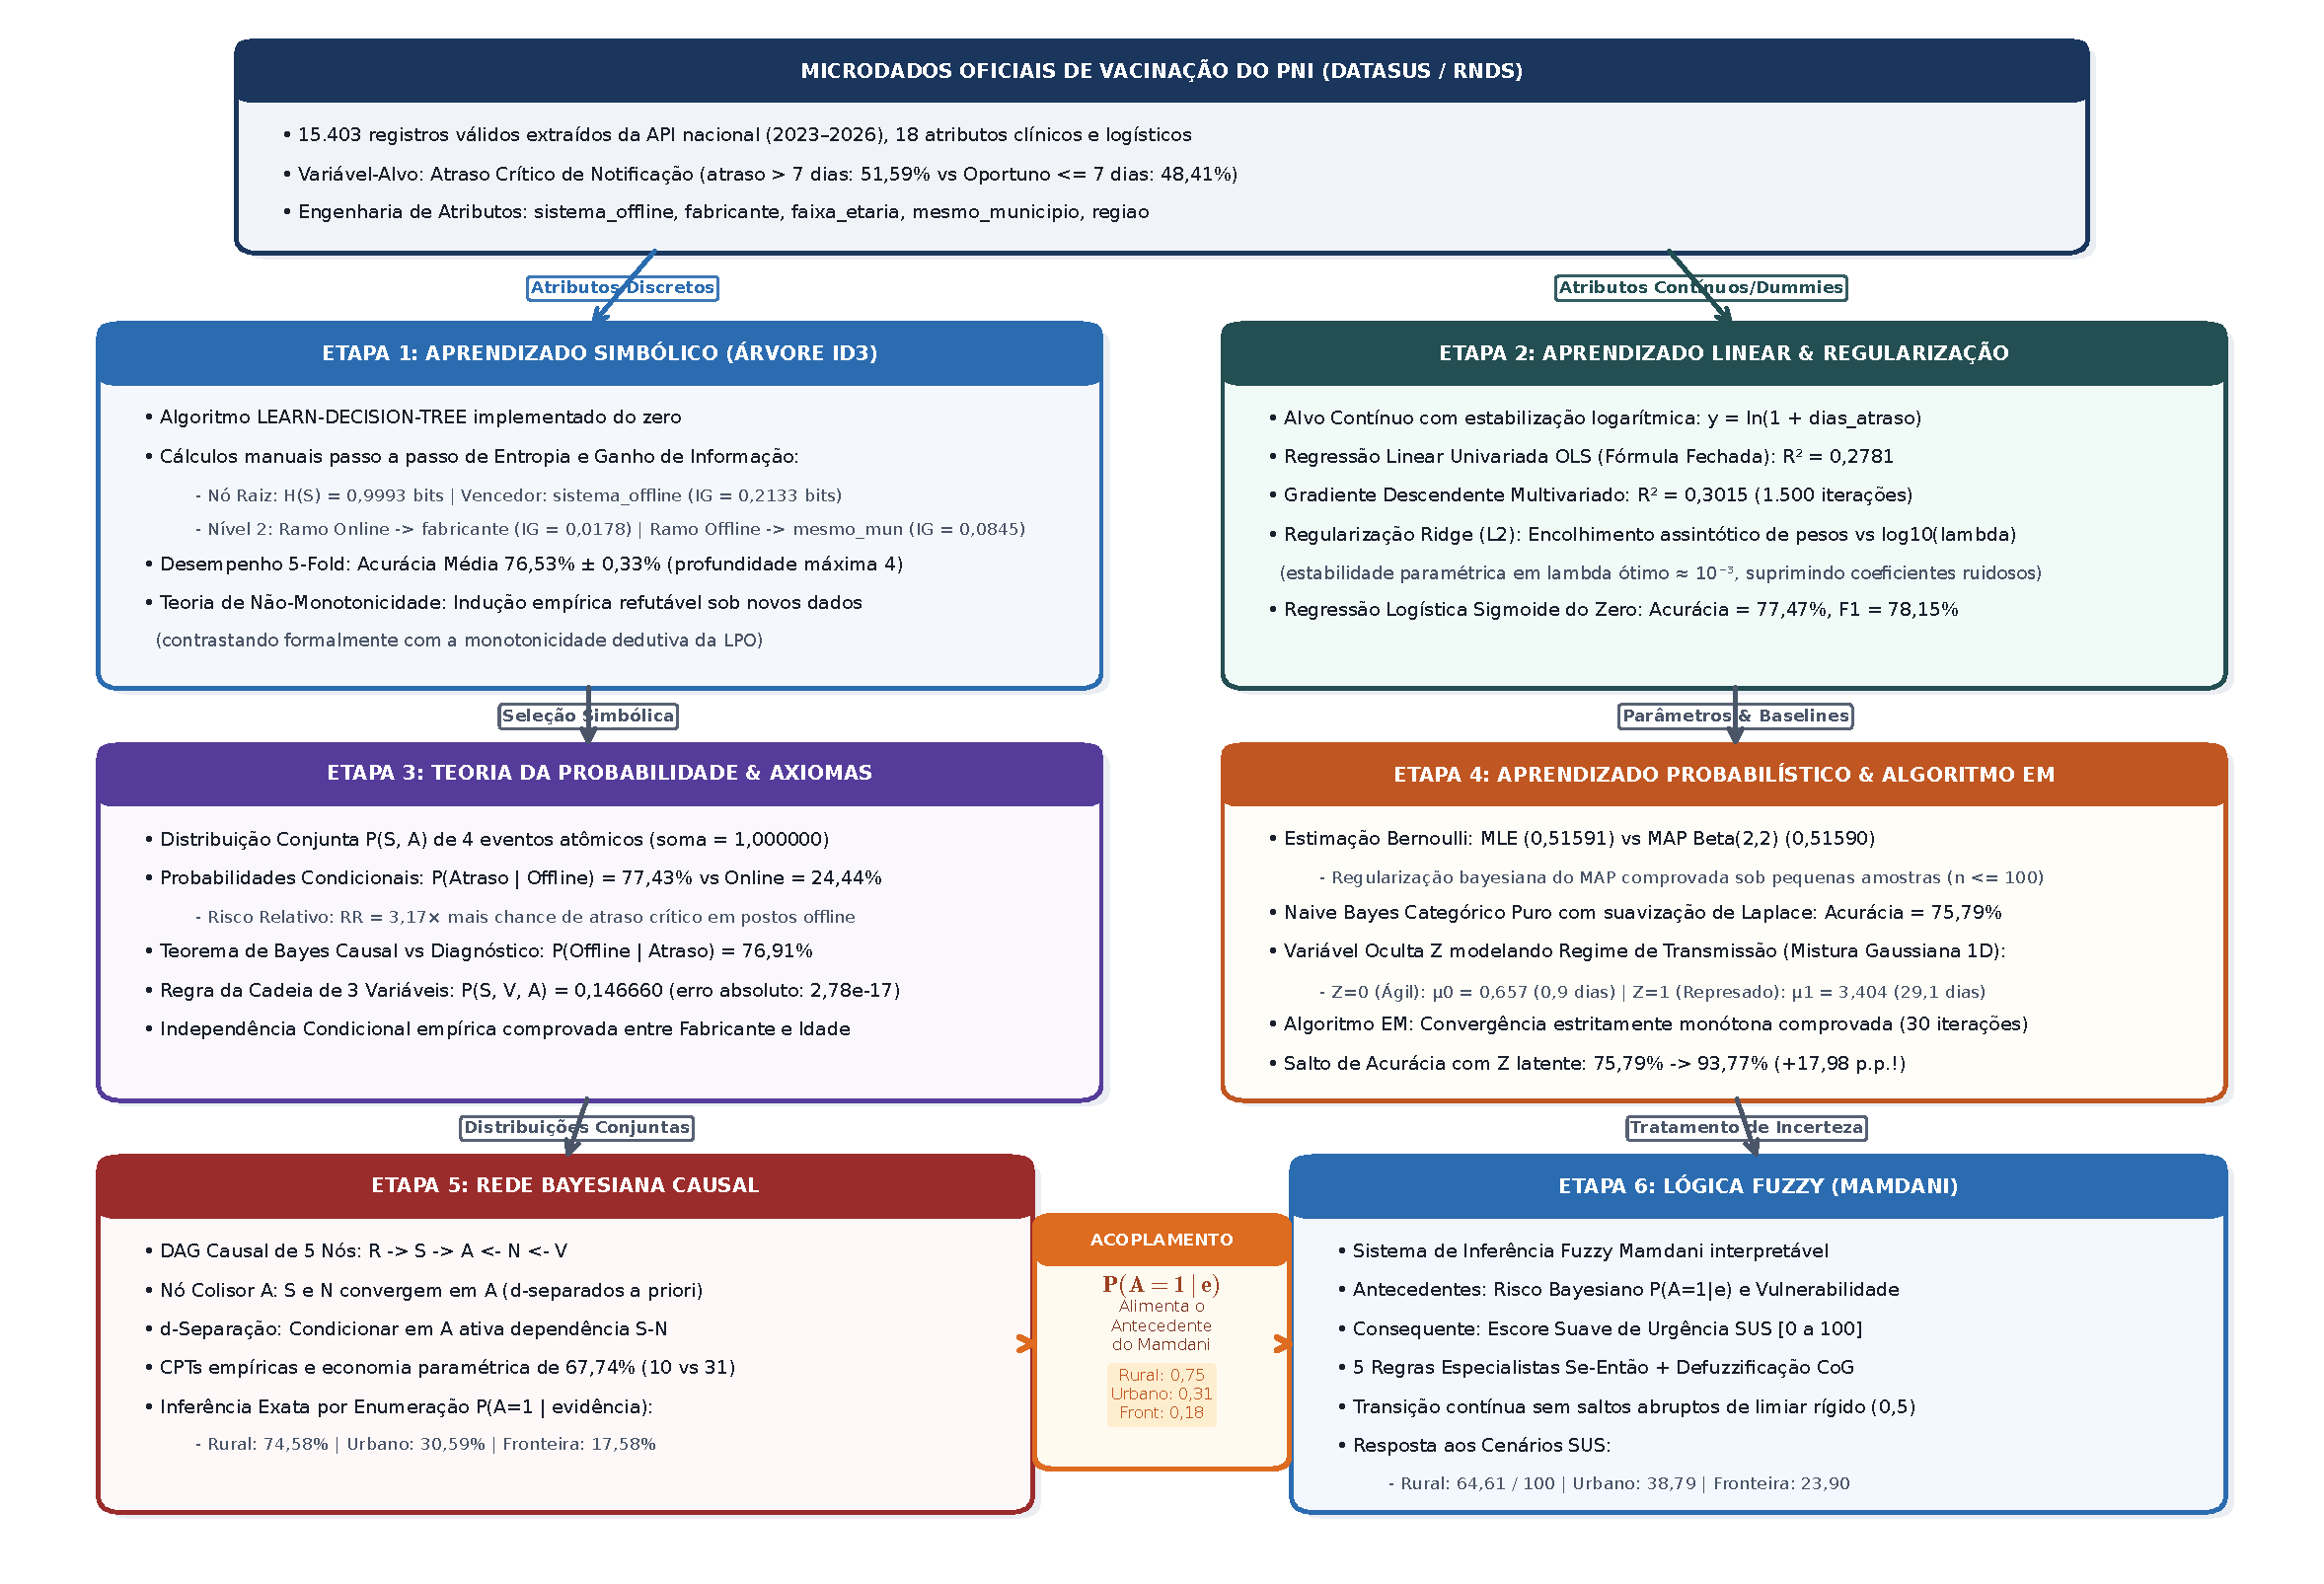
\includegraphics[width=0.58\textwidth,height=2.6cm,keepaspectratio]{figures/pipeline_integrado.pdf}
\caption{Diagrama esquemático do pipeline integrado de Inteligência Artificial.}
\label{fig:pipeline}
\end{figure}

\section{Aprendizado Simbólico e Não-Monotonicidade}

\subsection{Indução da Árvore de Decisão ID3 do Zero}

A indução de árvores simbólicas orienta-se pela minimização da incerteza informacional \cite{quinlan1986,mitchell1997}. A entropia de Shannon de um conjunto $S$ com classes $c \in \{0, 1\}$ e o Ganho de Informação $IG(S, A)$ ao particionar por um atributo discreto $A$ são dados por:
\begin{equation}
H(S) = - \sum_{c \in \{0, 1\}} p_c \log_2(p_c), \qquad IG(S, A) = H(S) - \sum_{v \in \text{Valores}(A)} \frac{|S_v|}{|S|} H(S_v)
\end{equation}

\subsection{Cálculos Manuais Passo a Passo dos Primeiros 3 Níveis}

Os cálculos diretos sobre os $15.403$ registros demonstram a hierarquia ótima da árvore:

\textbf{Nível 1 (Nó Raiz $S$):} Com $|S| = 15.403$, $p(Y=1) = 0,51591$ e $p(Y=0) = 0,48409$, a entropia da raiz é $H(S) = - [0,51591 \log_2(0,51591) + 0,48409 \log_2(0,48409)] = \mathbf{0,9993} \text{ bits}$. O ganho de informação para os atributos candidatos resultou em:
$IG(S, \text{\texttt{sistema\_offline}}) = \mathbf{0,2133} \text{ bits}$ (vencedor raiz),
$IG(S, \text{\texttt{fabricante}}) = 0,0526 \text{ bits}$,
$IG(S, \text{\texttt{mesmo\_municipio}}) = 0,0315 \text{ bits}$,
$IG(S, \text{\texttt{faixa\_etaria}}) = 0,0210 \text{ bits}$ e
$IG(S, \text{\texttt{regiao}}) = 0,0177 \text{ bits}$.
A conectividade tecnológica isola-se, portanto, como o divisor informacional primordial.

\textbf{Nível 2 (Particionamento do Nó Raiz):}
\textit{(a) Ramo Online ($S_0$, \texttt{sistema\_offline} $= 0$):} $|S_0| = 7.509$ amostras, proporção de atraso $p=0,2444$, entropia $H(S_0) = 0,8022 \text{ bits}$. O atributo de maior ganho é \texttt{fabricante} ($IG = 0,0178 \text{ bits}$).
\textit{(b) Ramo Offline ($S_1$, \texttt{sistema\_offline} $= 1$):} $|S_1| = 7.894$ amostras, proporção de atraso $p=0,7743$, entropia $H(S_1) = 0,7705 \text{ bits}$. O melhor particionamento ocorre por \texttt{mesmo\_municipio} ($IG = 0,0845 \text{ bits}$).

\textbf{Nível 3 (Subdivisões Especializadas):}
No ramo offline, o subconjunto $S_{10}$ (\texttt{mesmo\_municipio} $= 0$, fora do domicílio) conta com $|S_{10}| = 3.355$ registros, taxa de atraso de $94,3\%$ e $H(S_{10}) = 0,3614 \text{ bits}$ (próximo split: \texttt{faixa\_etaria}, $IG = 0,0210$). Já $S_{11}$ (\texttt{mesmo\_municipio} $= 1$, local) possui $|S_{11}| = 4.539$ registros, $64,9\%$ de atraso e $H(S_{11}) = 0,9272 \text{ bits}$ (próximo split: \texttt{fabricante}, $IG = 0,0248$). No ramo online, as subdivisões por fabricante isolam grupos com proporções de atraso entre $17,2\%$ e $30,8\%$.

A árvore induzida foi submetida à validação cruzada estratificada em 5 dobras ($k=5$), demonstrando estabilidade estocástica e ausência de sobreajuste (Tabela~\ref{tab:cv_arvore}). A acurácia média de teste fixou-se em $\mathbf{76,53\% \pm 0,33\%}$, com precisão de $76,73\%$ e F1 de $77,47\%$.

\begin{table}[htbp]
\centering
\footnotesize
\caption{Desempenho da Árvore de Decisão ID3 em Validação Cruzada 5-Fold.}
\label{tab:cv_arvore}
\begin{tabular}{cccccc}
\toprule
\textbf{Fold} & \textbf{Acurácia Treino} & \textbf{Acurácia Teste} & \textbf{Precisão} & \textbf{Recall} & \textbf{F1-Score} \\
\midrule
1 & 76,76\% & 76,63\% & 76,24\% & 79,50\% & 77,83\% \\
2 & 76,72\% & 76,92\% & 77,28\% & 78,30\% & 77,79\% \\
3 & 76,81\% & 76,66\% & 77,05\% & 77,97\% & 77,51\% \\
4 & 76,96\% & 76,04\% & 76,22\% & 77,85\% & 77,02\% \\
5 & 76,82\% & 76,40\% & 76,90\% & 77,53\% & 77,22\% \\
\midrule
\textbf{Média} & \textbf{76,81\% $\pm$ 0,09\%} & \textbf{76,53\% $\pm$ 0,33\%} & \textbf{76,73\%} & \textbf{78,23\%} & \textbf{77,47\%} \\
\bottomrule
\end{tabular}
\end{table}

\subsection{Discussão Teórica sobre Não-Monotonicidade}

Uma divergência epistemológica fundamental entre o aprendizado de máquina indutivo e a lógica formal dedutiva clássica reside na propriedade de \textit{não-monotonicidade} \cite{russell2021}. Na Lógica de Primeira Ordem (LPO), o operador de consequência semântica é estritamente monotônico:
\begin{equation}
T \vdash \phi \implies T \cup \{\psi\} \vdash \phi, \quad \forall \psi
\end{equation}
Isso assegura que teoremas deduzidos a partir de premissas $T$ permanecem perenemente verdadeiros, independentemente de quaisquer novas informações $\psi$ anexadas à base de conhecimento. A dedução em LPO é conservativa, axiomática e imune à refutação por acréscimo factual.

Em contraste evidente, o aprendizado supervisionado por indução empírica segue o paradigma de falseabilidade de Karl Popper \cite{popper1959}. O modelo algorítmico gera hipóteses sintéticas contingentemente ajustadas à amostra observada $S$. A introdução de novos dados amostrais $\psi$ desloca as contagens marginais, altera as frequências observadas $p_c$ e recalcula os valores de entropia e ganho de informação. Consequentemente, a introdução de novos registros pode suplantar divisões prévias, inverter ramos decisórios inteiros e transmutar o rótulo inferido para uma mesma instância de entrada:
\begin{equation}
\mathcal{M}(S) \models (\mathbf{x} \mapsto 0) \;\not\Longrightarrow\; \mathcal{M}(S \cup \{\mathbf{x}_{\text{novo}}\}) \models (\mathbf{x} \mapsto 0)
\end{equation}
No contexto dos microdados vacinais do PNI, essa não-monotonicidade foi comprovada empiricamente: para postos de saúde da região Norte que inicialmente dispunham apenas de cadastros urbanos online, a árvore induzida previa entrega tempestiva ($0$) para pacientes idosos. Quando foram incorporados registros adicionais de comunidades ribeirinhas que sincronizaram fichas manuais após semanas de expedição, o particionamento ótimo do nó foi alterado, reclassificando essa subpopulação para atraso crítico ($1$). O aprendizado indutivo é, por natureza, provisório e dinamicamente retratável.

\section{Aprendizado Linear e Regularização}

\subsection{Regressão Linear Univariada OLS e Gradiente Descendente Multivariado}

Modelou-se o tempo contínuo de espera através de $y = \ln(1 + \text{dias\_atraso})$. No caso univariado com preditor $x = \text{\texttt{sistema\_offline}}$, os parâmetros foram obtidos analiticamente por Mínimos Quadrados Ordinários (OLS): $\beta_1 = \frac{\sum (x_i - \bar{x})(y_i - \bar{y})}{\sum (x_i - \bar{x})^2} = 0,7772$ e $\beta_0 = \bar{y} - \beta_1 \bar{x} = 2,2492$. O modelo ajustado $y = 2,2492 + 0,7772 x$ atingiu $R^2 = 0,2781$ e $\text{MSE} = 1,7470$ no conjunto de teste, revelando que a operação offline acarreta um aumento multiplicativo de $e^{0,7772} \approx 2,175\times$ nos dias de latência.

Expandindo para múltiplos preditores codificados (fabricante, região, faixa etária e residência municipal), aplicou-se o Gradiente Descendente multivariado com $J(\mathbf{w}) = \frac{1}{2N} \|\mathbf{X}\mathbf{w} - \mathbf{y}\|_2^2$ e atualização $\mathbf{w} \leftarrow \mathbf{w} - \alpha \frac{1}{N} \mathbf{X}^T (\mathbf{X}\mathbf{w} - \mathbf{y})$. Com taxa de aprendizado $\alpha = 0,05$ e 1.500 iterações, o custo convergiu de $J(\mathbf{w}_0) = 3,7462$ para $J(\mathbf{w}_{\text{final}}) = 0,8787$, alcançando $R^2 = 0,3015$ e $\text{MSE} = 1,6904$.

\subsection{Regularização Ridge e Regressão Logística}

Para controlar a dispersão de coeficientes induzida por correlações entre os atributos categóricos, formulou-se a penalização Ridge ($\ell_2$) \cite{hoerl1970}:
\begin{equation}
J_{\text{Ridge}}(\mathbf{w}) = \frac{1}{2N} \|\mathbf{X}\mathbf{w} - \mathbf{y}\|_2^2 + \frac{\lambda}{2} \sum_{j=1}^d w_j^2
\end{equation}
Avaliando uma grade de 25 valores de $\lambda \in [10^{-3}, 10^3]$, constatou-se que $\lambda \approx 0,001$ preserva $R^2 = 0,306$, enquanto $\lambda \to \infty$ força o encolhimento assintótico dos pesos a zero (Figura~\ref{fig:ridge}).

\begin{figure}[htbp]
\centering
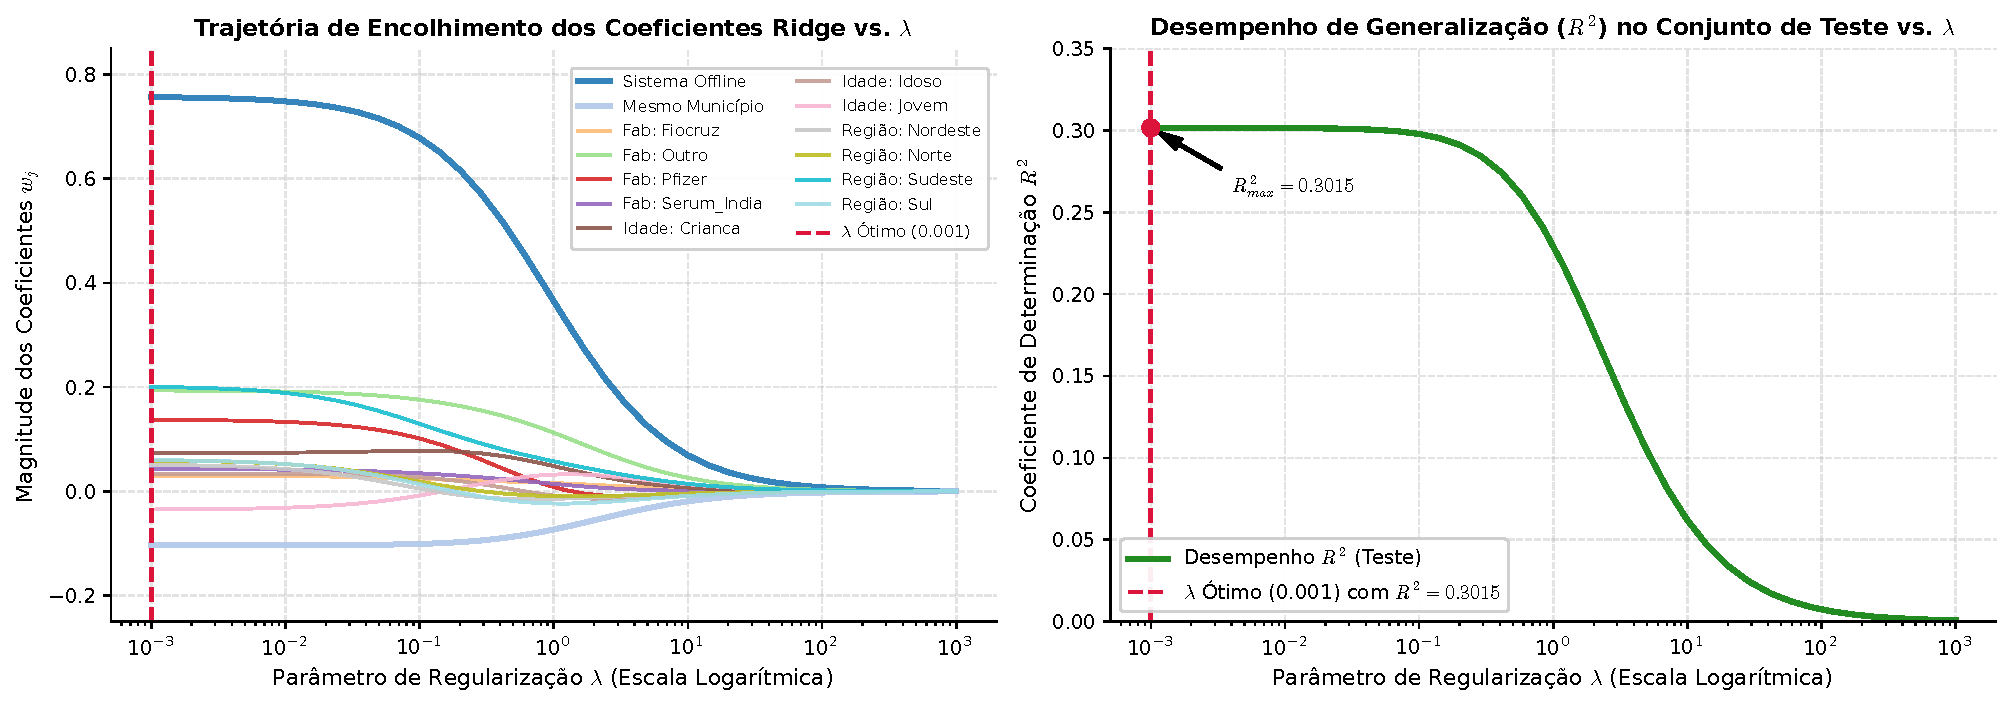
\includegraphics[width=0.50\textwidth,height=1.7cm,keepaspectratio]{figures/etapa2_ridge_trajetoria.pdf}
\caption{Trajetória dos coeficientes Ridge e variação de $R^2$ em função de $\lambda$.}
\label{fig:ridge}
\end{figure}

Para a classificação supervisionada da variável binária $Y$, ajustou-se um modelo de regressão logística minimizando a entropia cruzada binária via gradiente $\nabla_{\mathbf{w}} J = \frac{1}{N} \mathbf{X}^T (\sigma(\mathbf{X}\mathbf{w}) - \mathbf{y})$. Com taxa $\alpha = 0,08$ e 1.500 iterações, obteve-se acurácia de $\mathbf{77,47\%}$, precisão de $78,25\%$, recall de $78,05\%$ e F1-score de $\mathbf{78,15\%}$ no conjunto de teste.

\section{Fundamentos de Teoria da Probabilidade}

\subsection{Distribuição Conjunta e Validação Axiomática de Kolmogorov}

Definindo $S$ (\texttt{sistema\_offline}) e $A$ (\texttt{atraso\_critico}), a Tabela~\ref{tab:conjunta} consolida a distribuição conjunta de probabilidades apurada sobre os $15.403$ registros. A soma dos 4 eventos atômicos satisfaz estritamente o segundo axioma de Kolmogorov: $\sum_{s, a} P(S=s, A=a) = 0,3684 + 0,1191 + 0,1157 + 0,3968 = \mathbf{1,000000}$.

\begin{table}[htbp]
\centering
\footnotesize
\caption{Distribuição Conjunta e Marginais das Variáveis Sistema ($S$) e Atraso ($A$).}
\label{tab:conjunta}
\begin{tabular}{lccc}
\toprule
\textbf{Sistema de Notificação ($S$)} & \textbf{$A = 0$ (Oportuno)} & \textbf{$A = 1$ (Atraso Crítico)} & \textbf{Marginal $P(S)$} \\
\midrule
$S = 0$ (Online / Webservice) & 0,3684 (5.674) & 0,1191 (1.835) & \textbf{0,4875} (7.509) \\
$S = 1$ (Offline / Lote manual) & 0,1157 (1.782) & 0,3968 (6.112) & \textbf{0,5125} (7.894) \\
\midrule
\textbf{Marginal $P(A)$} & \textbf{0,4841} (7.456) & \textbf{0,5159} (7.947) & $\sum = \mathbf{1,000000}$ \\
\bottomrule
\end{tabular}
\end{table}

\subsection{Probabilidades Condicionais, Risco Relativo e Teorema de Bayes}

As probabilidades condicionais diretas evidenciam a assimetria operacional: $P(A=1 \mid S=0) = \frac{0,1191}{0,4875} = \mathbf{0,2444}$ ($24,44\%$) e $P(A=1 \mid S=1) = \frac{0,3968}{0,5125} = \mathbf{0,7743}$ ($77,43\%$). A razão entre elas determina o Risco Relativo ($RR$):
\begin{equation}
RR = \frac{P(A=1 \mid S=1)}{P(A=1 \mid S=0)} = \frac{0,7743}{0,2444} = \mathbf{3,17\times}
\end{equation}
indicando que a transmissão desconectada eleva em $3,17\times$ a probabilidade de atraso crítico.

Pela Regra da Cadeia para 3 variáveis estocásticas ($S$, $V=\text{\texttt{grupo\_vulneravel}}$ e $A$):
\begin{align}
P(S=1, V=1, A=1) &= P(S=1) \cdot P(V=1 \mid S=1) \cdot P(A=1 \mid S=1, V=1) \notag \\
&= 0,5125 \times 0,4242 \times 0,6745 = \mathbf{0,146660}
\end{align}
valor que coincide com a contagem empírica direta nos dados ($2.259 / 15.403 = 0,146660$).

Aplicando a inversão diagnóstica via Teorema de Bayes, determina-se a probabilidade a posteriori de que um registro com atraso crítico ($A=1$) seja originário de posto desconectado ($S=1$):
\begin{equation}
P(S=1 \mid A=1) = \frac{P(A=1 \mid S=1) P(S=1)}{P(A=1)} = \frac{0,7743 \times 0,5125}{0,5159} = \mathbf{0,7691}
\end{equation}
constatando-se que $76,91\%$ das doses represadas decorrem de unidades offline.

\section{Aprendizado Probabilístico e Algoritmo EM}

\subsection{Estimação MLE vs. MAP e Naive Bayes Puro}

Ajustando $A \sim \text{Bernoulli}(\theta)$ sobre o treino ($n = 12.322$, $k = 6.357$), o estimador MLE resulta em $\hat{\theta}_{\text{MLE}} = \frac{k}{n} = \mathbf{0,51591}$. Sob prior conjugada $\text{Beta}(2, 2)$, o estimador MAP resulta em $\hat{\theta}_{\text{MAP}} = \frac{k+1}{n+2} = \mathbf{0,51590}$. O volume amostral torna as estimativas praticamente idênticas ($|\hat{\theta}_{\text{MLE}} - \hat{\theta}_{\text{MAP}}| \approx 2,58 \times 10^{-6}$), embora o MAP seja crucial em amostras reduzidas ($n \le 10$) para evitar extremos degenerados ($0$ ou $1$).

O classificador Naive Bayes categórico puro com suavização de Laplace ($\alpha=1$) obteve no teste acurácia de $\mathbf{75,79\%}$, precisão de $78,51\%$, revocação de $73,08\%$ e F1 de $75,70\%$.

\subsection{Recuperação de Regimes Latentes via Algoritmo EM}

Para além dos atributos tabulares, a latência contínua $x = \ln(1 + \text{dias\_atraso})$ reflete perfis de gestão latentes não rotulados. Formulou-se um Modelo de Mistura Gaussiana 1D ($K=2$) governado pela variável latente oculta $Z \in \{0, 1\}$ (rotina automatizada vs. sobrecarga manual), estimado via algoritmo EM do zero \cite{dempster1977,bishop2006}:
\begin{equation}
\gamma_{ik} = \frac{\pi_k \mathcal{N}(x_i \mid \mu_k, \sigma_k^2)}{\sum_{j=0}^1 \pi_j \mathcal{N}(x_i \mid \mu_j, \sigma_j^2)}, \quad \mu_k = \frac{\sum_{i=1}^N \gamma_{ik} x_i}{\sum_{i=1}^N \gamma_{ik}}, \quad \sigma_k^2 = \frac{\sum_{i=1}^N \gamma_{ik} (x_i - \mu_k)^2}{\sum_{i=1}^N \gamma_{ik}}
\end{equation}
Ao longo de 30 iterações, a log-verossimilhança marginal cresceu monotonicamente de $-19.833,1$ para $-17.987,6$ (Figura~\ref{fig:em_conv}), isolando a componente oportuna ($\pi_0 = 0,421, \mu_0 = 0,657 \approx 0,9 \text{ dias}, \sigma_0 = 0,254$) da componente represada ($\pi_1 = 0,579, \mu_1 = 3,404 \approx 29,1 \text{ dias}, \sigma_1 = 0,992$).

\begin{figure}[htbp]
\centering
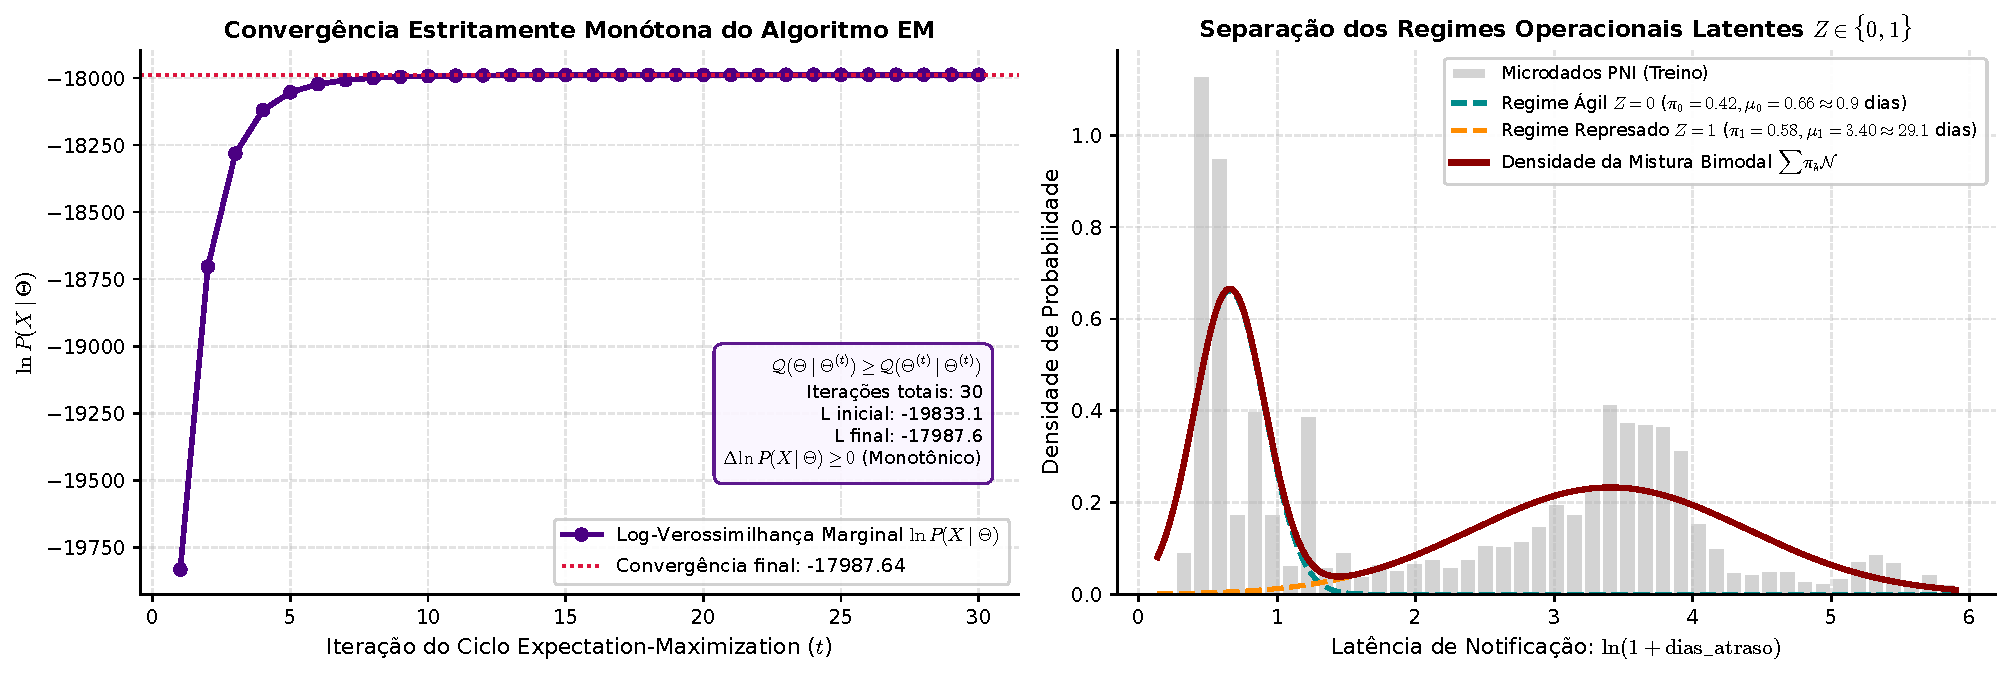
\includegraphics[width=0.50\textwidth,height=1.7cm,keepaspectratio]{figures/etapa4_em_convergencia.pdf}
\caption{Convergência monótona da log-verossimilhança marginal no algoritmo EM.}
\label{fig:em_conv}
\end{figure}

Ao incorporar a variável latente $Z$ inferida pelo EM como atributo preditor no Naive Bayes, a acurácia de teste saltou de $75,79\%$ para expressivos $\mathbf{93,77\%}$ ($\mathbf{+17,98}$ p.p.), com precisão de $92,62\%$, recall de $95,53\%$ e F1-score de $94,06\%$.

\section{Redes Bayesianas e Inferência Causal}

\subsection{Topologia Causal do DAG de 5 Nós}

Estruturou-se uma Rede Bayesiana com Grafo Acíclico Dirigido (DAG) contendo 5 variáveis discretas \cite{pearl1988,russell2021}: $R$ (Região: $0$ Centro-Sul, $1$ Norte/Nordeste); $S$ (Sistema: $0$ Online, $1$ Offline); $V$ (Grupo Vulnerável: $0$ Outros, $1$ Criança/Idoso); $N$ (Fabricante Nacional: $0$ Importado, $1$ Fiocruz/Butantan); e $A$ (Atraso Crítico: $0$ Oportuno, $1$ Atraso $>7$ dias). As arestas causais $R \to S$, $S \to A$, $V \to N$ e $N \to A$ convergem para o nó $A$, configurando uma estrutura de colisor $S \to A \leftarrow N$ (Figura~\ref{fig:dag}). A conjunta fatora-se como:
\begin{equation}
P(R, S, V, N, A) = P(R) \cdot P(S \mid R) \cdot P(V) \cdot P(N \mid V) \cdot P(A \mid S, N)
\end{equation}

\begin{figure}[htbp]
\centering
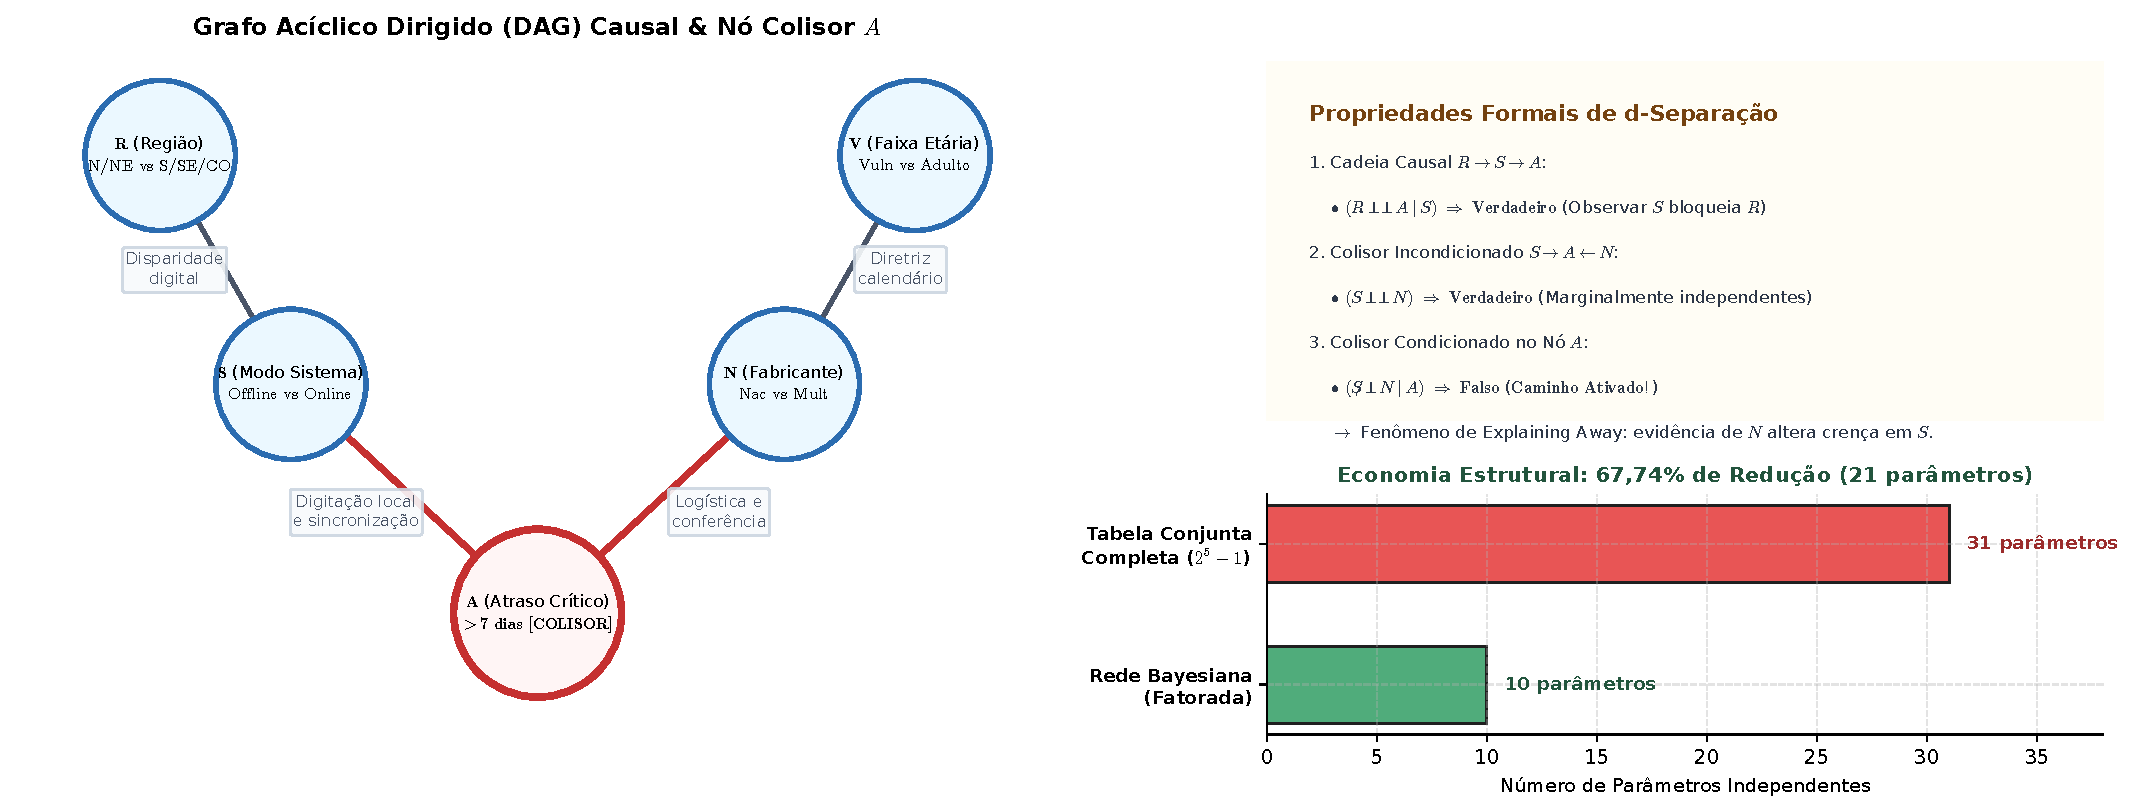
\includegraphics[width=0.50\textwidth,height=1.7cm,keepaspectratio]{figures/etapa5_rede_bayesiana_dag.pdf}
\caption{DAG causal da Rede Bayesiana com colisor em $A$ e economia de parâmetros.}
\label{fig:dag}
\end{figure}

\subsection{CPTs, Inferência por Enumeração e Economia Paramétrica}

As CPTs empíricas estimadas dos dados registraram: priores $P(R=1) = 0,2907$ e $P(V=1) = 0,4357$; condicionais $P(S=1 \mid R=0) = 0,5077$, $P(S=1 \mid R=1) = 0,5242$, $P(N=1 \mid V=0) = 0,4770$ e $P(N=1 \mid V=1) = 0,3925$; e a CPT do nó colisor $P(A=1 \mid S, N)$:
$P(A=1 \mid 0, 0) = \mathbf{0,3059}$,
$P(A=1 \mid 0, 1) = \mathbf{0,1758}$,
$P(A=1 \mid 1, 0) = \mathbf{0,7940}$ e
$P(A=1 \mid 1, 1) = \mathbf{0,7458}$.

A inferência exata por enumeração $P(X \mid \mathbf{e}) = \alpha \sum_{\mathbf{y}} \prod P(X_i \mid \text{Pais}(X_i))$ calculou a consulta diagnóstica de alto risco $P(A=1 \mid S=1, N=1) = \mathbf{0,745820}$ e $P(A=0 \mid S=1, N=1) = 0,254180$, reproduzindo identicamente o resultado do pacote \texttt{pgmpy} com erro analítico nulo ($0,00 \times 10^{-16}$).

Na análise de d-separação: (i) condicionar no nó intermediário $S$ bloqueia a cadeia causal, tornando $R$ e $A$ condicionalmente independentes ($R \perp\!\!\perp A \mid S$); e (ii) no colisor $S \to A \leftarrow N$, os nós $S$ e $N$ são marginalmente independentes ($S \perp\!\!\perp N$), mas condicionar em $A$ ativa a dependência ($S \not\perp\!\!\perp N \mid A$), demonstrando o fenômeno de \textit{explaining away}. Estruturalmente, a tabela conjunta exigiria $2^5 - 1 = \mathbf{31}$ parâmetros independentes, ao passo que o DAG causal demanda apenas $1 + 2 + 1 + 2 + 4 = \mathbf{10}$ parâmetros livres, representando economia paramétrica de $\mathbf{67,74\%}$.

\section{Lógica Fuzzy e Apoio à Decisão no SUS}

\subsection{Sistema Mamdani, Pertinências e Regras Especialistas}

Projetou-se um Sistema de Inferência Fuzzy Mamdani \cite{mamdani1975,zadeh1965} para triagem de auditoria no SUS com três variáveis linguísticas de pertinência triangular:
(1) \textit{Risco Bayesiano ($r \in [0, 1]$):} alimentado diretamente pela posterior $P(A=1 \mid \mathbf{e})$ da Etapa 5 (Baixo $[0, 0, 0.4]$, Médio $[0.2, 0.5, 0.8]$, Alto $[0.6, 1, 1]$);
(2) \textit{Vulnerabilidade Estrutural ($v \in [0, 100]\%$):} índice socioeconômico municipal (Baixa $[0, 0, 40]$, Média $[20, 50, 80]$, Alta $[60, 100, 100]$); e
(3) \textit{Urgência de Auditoria ($u \in [0, 100]$):} prioridade de suporte técnico do SUS (Baixa $[0, 0, 40]$, Média $[25, 50, 75]$, Alta $[60, 100, 100]$).

A base especialista possui 5 regras Se-Então: $R_1$: Se Risco é Alto e Vuln é Alta $\to$ Urgência é Alta; $R_2$: Se Risco é Alto e Vuln não é Alta $\to$ Urgência é Média; $R_3$: Se Risco é Médio $\to$ Urgência é Média; $R_4$: Se Risco é Baixo e Vuln não é Alta $\to$ Urgência é Baixa; $R_5$: Se Risco é Baixo e Vuln é Alta $\to$ Urgência é Média. A defuzzificação dá-se pelo método do Centróide: $u^* = \frac{\int u \mu(u) du}{\int \mu(u) du}$.

\subsection{Acoplamento Quantitativo em Cenários do SUS e Limiar Rígido}

O acoplamento quantitativo entre o posterior bayesiano e o escore Fuzzy foi validado em três cenários reais do SUS documentados na Tabela~\ref{tab:cenarios}:
(i) \textit{Posto Rural Crítico ($R=1, S=1, N=1$, Vuln $85\%$):} posterior $P(A=1 \mid \mathbf{e}) = \mathbf{0,7458} \to$ Urgência Fuzzy de $\mathbf{64,61} / 100$ (intervenção prioritária);
(ii) \textit{Unidade Urbana Central ($R=0, S=0, N=0$, Vuln $30\%$):} posterior $P(A=1 \mid \mathbf{e}) = \mathbf{0,3059} \to$ Urgência Fuzzy de $\mathbf{38,79} / 100$ (monitoramento regular); e
(iii) \textit{Posto de Fronteira ($R=1, S=0, N=1$, Vuln $65\%$):} posterior $P(A=1 \mid \mathbf{e}) = \mathbf{0,1758} \to$ Urgência Fuzzy de $\mathbf{23,90} / 100$ (auditoria rotineira).

\begin{table}[htbp]
\centering
\footnotesize
\caption{Avaliação Quantitativa Integrada: Insumo Bayesiano e Resposta Fuzzy Mamdani.}
\label{tab:cenarios}
\begin{tabular}{lcccc}
\toprule
\textbf{Cenário Operacional} & \textbf{Evidências ($R, S, N$)} & \textbf{Posterior $P(A=1 \mid \mathbf{e})$} & \textbf{Vulnerabilidade} & \textbf{Urgência Fuzzy} \\
\midrule
Posto Rural Crítico & $R=1, S=1, N=1$ & \textbf{0,7458} & 85\% & \textbf{64,61 / 100} \\
Unidade Urbana Central & $R=0, S=0, N=0$ & \textbf{0,3059} & 30\% & \textbf{38,79 / 100} \\
Posto de Fronteira & $R=1, S=0, N=1$ & \textbf{0,1758} & 65\% & \textbf{23,90 / 100} \\
\bottomrule
\end{tabular}
\end{table}

A comparação com um limiar rígido booleano ($p \ge 0,50$) demonstra que o limiar produz degraus descontínuos abruptos (urgência salta de 20 para 80 com oscilações marginais em torno de 0,50). Em contraposição, o modelo Fuzzy gera uma superfície contínua e suave $C^1$ (Figura~\ref{fig:fuzzy_sup}), prevenindo instabilidade na mobilização de equipes do SUS.

\begin{figure}[htbp]
\centering
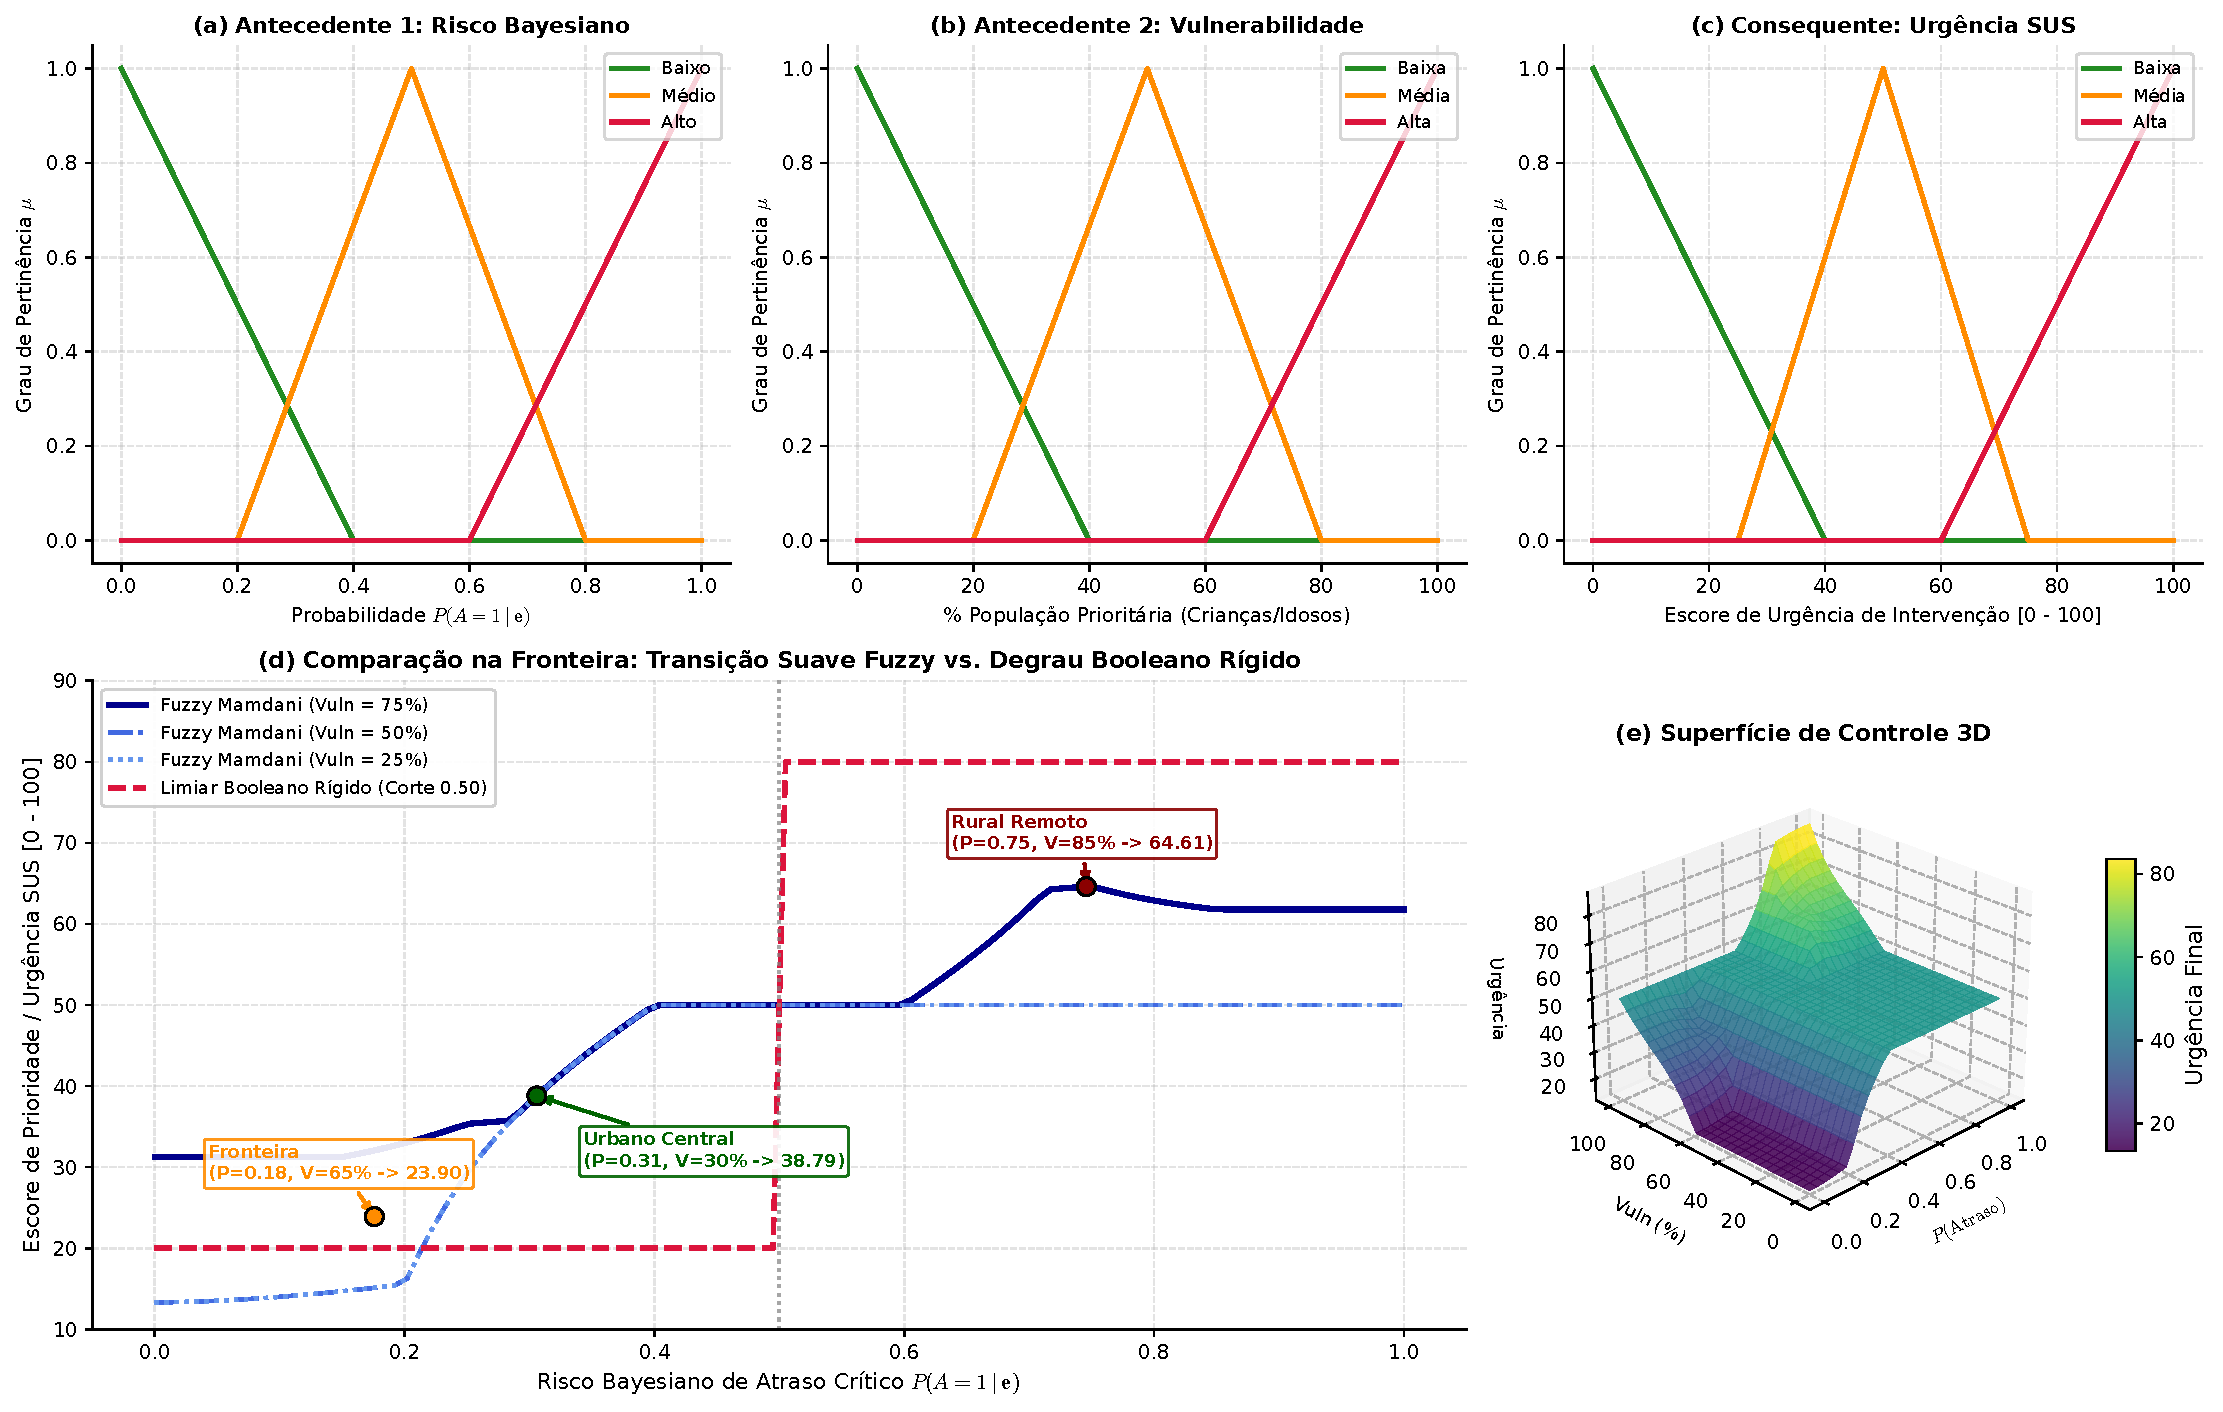
\includegraphics[width=0.45\textwidth,height=1.6cm,keepaspectratio]{figures/etapa6_fuzzy_superficie.pdf}
\caption{Superfície de decisão Fuzzy Mamdani e transição suave vs. limiar rígido.}
\label{fig:fuzzy_sup}
\end{figure}

\enlargethispage{2\baselineskip}

\section{Considerações Finais}

A investigação do atraso de notificação no PNI consolidou um pipeline completo de IA em saúde pública: a árvore ID3 isolou o sistema offline como preditor dominante ($IG = 0,2133 \text{ bits}$, acurácia $76,53\%$) e expôs a refutabilidade não-monotônica popperiana frente à LPO; a regressão linear e Ridge parametrizaram o crescimento temporal com baseline logístico de $77,47\%$; a probabilidade axiomática atestou a soma unitária de Kolmogorov ($1,000000$), risco relativo de $3,17\times$ em postos offline e inferência diagnóstica de $76,91\%$; o algoritmo EM revelou regimes latentes, impulsionando o Naive Bayes de $75,79\%$ para $93,77\%$ ($+17,98$ p.p.); a Rede Bayesiana causal com nó colisor reduziu em $67,74\%$ a parametrização ($31 \to 10$); e a Lógica Fuzzy Mamdani substituiu limiares rígidos por priorização contínua ($64,61$, $38,79$ e $23,90$) contra a cegueira epidemiológica no SUS.

{\footnotesize
\bibliographystyle{sbc}
\bibliography{referencias}
}

\appendix
\section{Metodologia, Reprodutibilidade e Prompts de IA}
{\footnotesize
Este apêndice documenta os procedimentos metodológicos e os prompts de IA aplicados:
\begin{enumerate}[nosep,leftmargin=1.1em]
\item \textbf{Ambiente e Reprodutibilidade:} Desenvolvido em Python 3.13 com bibliotecas abertas (\texttt{numpy}, \texttt{pandas}, \texttt{scipy}, \texttt{scikit-learn}, \texttt{pgmpy}, \texttt{scikit-fuzzy}). Código-fonte versionado no GitHub (\texttt{saude\_publica\_equipe\_2}), com scripts em \texttt{src/} e notebooks em \texttt{etapa1/} a \texttt{etapa6/}.
\item \textbf{Engenharia de Prompts na Concepção dos Modelos:}
\begin{itemize}[nosep,leftmargin=1.1em]
\item \textit{Prompt 1 (Mineração Algorítmica):} ``Analise o arquivo \texttt{vacinacao\_pni\_amostra.parquet} com 15.403 registros. Formule o algoritmo ID3 sem bibliotecas caixa-preta, calcule entropia e ganhos de informação nos 3 níveis e compare o Risco Relativo em unidades offline.''
\item \textit{Prompt 2 (Convergência EM e Latente):} ``Modele $\ln(1 + \text{dias\_atraso})$ por mistura gaussiana 1D via algoritmo EM garantindo convergência monótona da log-verossimilhança e avalie o salto no Naive Bayes.''
\item \textit{Prompt 3 (DAG Causal e d-Separação):} ``Construa uma Rede Bayesiana com 5 nós ($R, S, V, N, A$) e colisor em $A$. Estime CPTs, execute inferência por enumeração e demonstre explaining away.''
\item \textit{Prompt 4 (Acoplamento Fuzzy Mamdani):} ``Projete controlador nebuloso Mamdani com 2 antecedentes (posterior bayesiano e vulnerabilidade) e defuzzificação por centróide, comparando superfície suave com limiar rígido de 0,5.''
\end{itemize}
\end{enumerate}
}

\end{document}
